\chapter{Background}
\label{chap:background}

%\newglossaryentry{vr}{name={VR},description={virtual reality}}

Throughout our society's history, advancements in technology have been a prominent factor that separate generations from those proceeding. Recently, our development and discovery of new and exciting technologies has increased at exponential paces since the invention of the computer. As well, with these new technologies our society has been shifting and developing in many different aspects. One of the more fascinating technologies that have arisen in this period of rapid development is known as VR. This particular technology aims to immerse users further into the conceptual world of computing and serves to trick the user into believing in a virtual world that doesn't really exist. This is most often done through a device known as a Head Mounted Display (HMD). The first HMD was created in the early 1960s, and since then computer scientists have been trying to perfect the technology in order to create fully realistic virtual worlds that instill a perfect sense of presence.

\section{History of VR}
\label{sec:vrhistory}

VR is a technology with a particularly interesting past. In many ways VR has gone through waves of popularity in the public sphere, yet ever since its onset it has remained diligently used in certain circles. While we are currently experiencing a surge in VR adoption and advancement, the technology has often gone through periods of very little development since its invention. Furthermore, in different eras VR has been seen in different realms of use, from training to gaming.

\subsection{Headsight}
\label{sec:history1}

While a handful of patents existed for HMDs prior to 1960, the first HMD didn't appear until 1961. This HMD was developed by Philco Corporation by Comeau and Bryan, and was aptly named the Headsight \cite{steve_2008}. This rudimentary HMD used a magnetic tracking system with a single CRT monitor mounted into a bulky helmet, and moreover showed a remote video. In the early days of HMD technology, all HMDs followed the same basic design as the Headsight project, that is they all remotely "streamed" video to the HMDs which merely showed the video projections. Many early HMDs, including Headsight, allowed for head tracking which could remotely move the camera transmitting the video feed, allowing for a user to look around an entire scene. The first major application for Headsight was used by Bell Helicopter Company to provide pilots with an alternate video see-through view \cite{michael_emerging_2006}. 

\subsection{Ivan Sutherland}
\label{sec:history2}

As mentioned, early HMD technology such as the Headsight merely passed video through to a CRT inside a helmet. It wasn't until 1965 that Ivan Sutherland demonstrated the first tethered display system which would allow computer-generated images to be overplayed inside an HMD system. In his case, Sutherland's first project was called "Sword of Damocles", and it featured a set of CRT optical relays for each individual eye, allowing each eye to observe computer generated imagery \cite{steve_2008}. Moreover, Sutherland's design allowed for these computer generated graphics to be superimposed onto the real environment surrounding the user. As the viewer moved around, the computer imagery would appear stable within the real environment. On the whole, Sutherland was the first to envision what he named the "Ultimate Display". This vision would guide almost all future development in VR, and it laid down three core tenants of VR technology. According to Sutherland, in order for VR to be a successful technology, VR worlds must appear real to any observer, a computer must maintain the world in real time,  and manipulation of VR objects must seem realistic \cite{packer_multimedia:_2001}.

\subsection{1965-1980s}
\label{sec:history3}

With the tenants established by Sutherland, VR development would continue on a steady pace throughout the rest of the 1960s and well into the 1980s. During this time the primary funders, adopters, and users of VR technology were American military and scientific sponsors. For the most part, the major funders were the NSF, NASA, and the Department of Defense. The technology was mainly used for vehicle simulations, and the technology stayed out of the public eye. NASA would use the technology in their BOOM display to help aid astronauts in future space walks. On the other hand, the military used VR HMDs for training purposes. The technology was appealing to the military because it provided environments to train normally high risk and high stress skills, such as combat and field medicine. VR proved an invaluable tool for the military by allowing training to take place under pressure with no risk in failure. As well, both the military and the NSF used the technology to help with pilot training, allowing for pilots to train without the risk or need of expensive aircraft.

\subsection{Michael McGreevy}
\label{sec:history4}

Much like Sutherland in the 1960s, VR would again shift course in the mid 1980s due to the visionary work of one man, Michael McGreevy. McGreevy saw VR in a new light, and for the first time sought to integrate the technology into a growing academic subfield of computer science known as Human Computer Interaction (HCI). This new academic interest in VR fueled future research in the technology, and even today HCI still plays a primary role in VR research. Additionally, McGreevy was the first person to coin the term "Virtual Reality" in 1987, and the term has been in use ever since.

\subsection{1990s}
\label{sec:history5}

VR technology largely stayed out of the public eye until the 1990s, when media would aggressively latch onto the technology for better or for worse. In many ways the vast amount of media attention that VR received in the 1990s was related to the onset of video gaming. For example, the popular PC gaming magazine Computer Gaming World predicted that affordable VR HMDs would be widely available for public use in 1994. This unrealistic hype generated huge expectations that would be crushed when the public realized the limitations of the technology at the time. Large gaming companies like Sega and Nintendo both attempted to introduce VR onto their gaming platforms, but both failed spectacularly. Soon public interest began to fall, and again the technology returned to the private sphere of military and science uses for the most part.

\section{Current VR Development}
\label{sec:vrinnovations}

While the technology behind VR has been steadily advancing over the years, it wasn't until 2012 that VR finally began a surge in popularity, adoption, and advancement. Largely due to the work of one company, Oculus VR, and one man, Palmer Luckey, VR has been advancing at unprecedented rates since 2012. The media attachment to VR has returned from the 1990s, but this time the technology is far and above anyone's imagination. For the first time VR has entered into a public spotlight, and at every turn it continues to blow away any and all expectations of what VR is capable of.

\subsection{Oculus Rift}
\label{sec:oculuisvr}

\begin{figure}
  \centering
  %\begin{picture}
  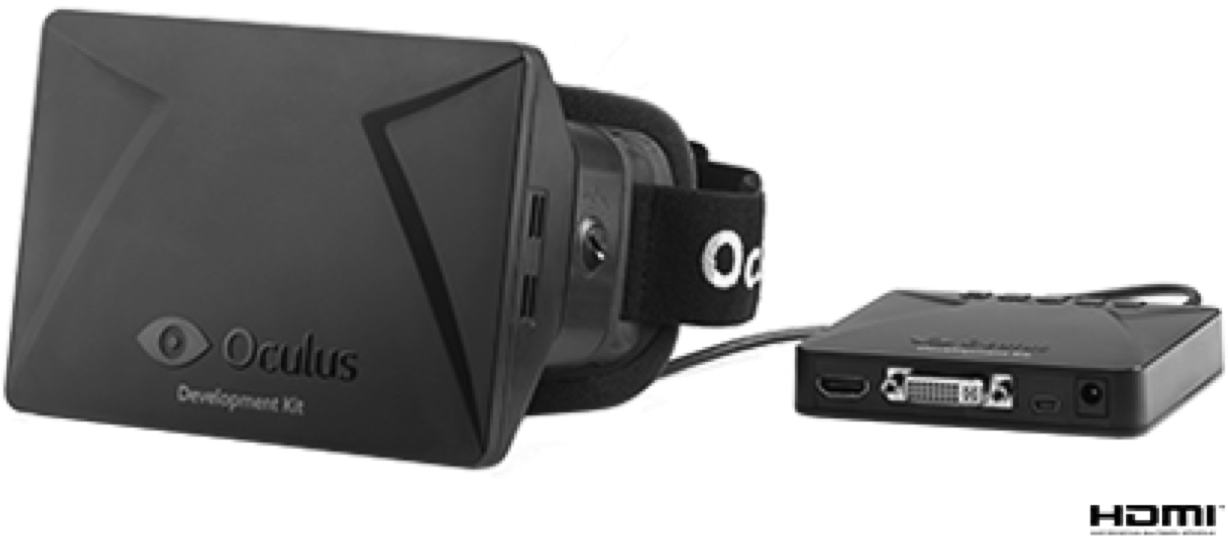
\includegraphics[scale=.5]{img_dk1}
  %\end{picture}
  \caption{Oculus Rift DK1 and control unit.}
  \label{figure:f_dk1}
\end{figure}
%Figure~\ref{figure:f_dk1}

In 2012, Palmer Luckey had one of the world's largest private collections of HMDs. He was a young man (only 19 at the time) obsessed with a technology that was in every way flawed. However, he was able to look past the flaws and envision a realistic HMD that could be built with technology available at the time, and would be able to provide a VR setting with a level of presence that had never been seen before. Luckey took his frustrations in the HMDs available at the time, and began building prototypes for a new era of HMDs. His earliest prototypes explored features such as 3D stereoscopy, wireless streaming, large field-of-views (up to 270 degrees), while at the same time cutting down on the bulkiness of the HMD with each iteration. By the time he was on his 6th prototype he thought he had built a proof of concept that would interest a niche market of HMD enthusiasts. Using this prototype he created his own company, Oculus VR, and launched a Kickstarter campaign to raise money in order to build and distribute the HMDs.

Luckey originally thought he would only interest around 100 investors in his Kickstarter campaign, and appropriately set a goal to raise \$250,000. However, perhaps through the interest of high profile investors such as John Carmack (id Software), and Gabe Newall (Valve), Luckey found that his Kickstarter goal would be far surpassed. In fact, his Kickstarter would go on to become one of the most overly funded Kickstarter campaigns of all time, as it raised 974\% of its original goal, or a total sum of \$2.4 million dollars. Due to its Kickstarter, Oculus VR soon became the world's leading developer in VR technologies and has become the face of modern day VR. 

\begin{figure}
  \centering
  %\begin{picture}
  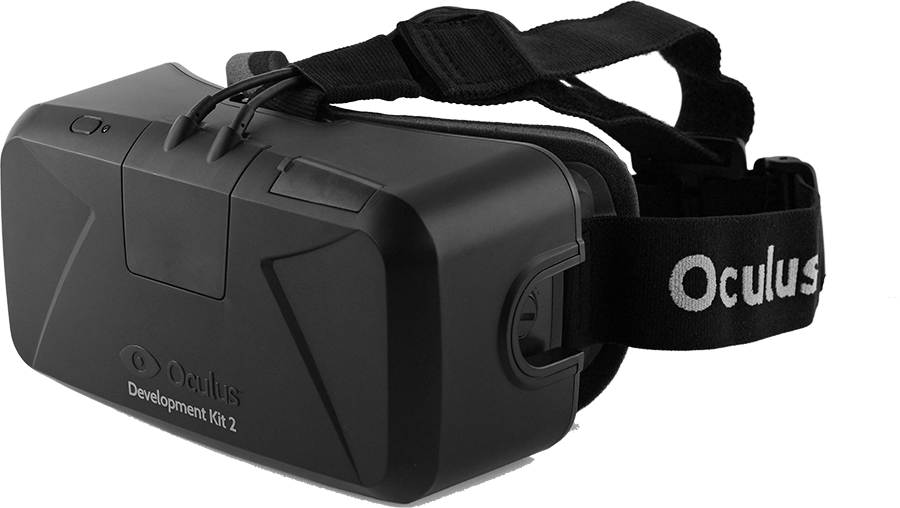
\includegraphics[scale=.5]{img_dk2}
  %\end{picture}
  \caption{Oculus Rift DK2 and tracking camera.}
  \label{figure:f_dk2}
\end{figure}

As a result of the Kickstarter, Oculus VR used its massive influx of funds to develop its first widely available VR HMD which was sent out to Kickstarter backers and available for sale directly to developers on the Oculus VR website in late 2012. This HMD was known as the Oculus Rift Development Kit 1 (DK1), and emerged as the first ever widely successful HMD. The DK1 boasted a 7 inch screen, with a resolution of 1280x800 (16:10), which allowed for a single eye resolution of 640x800. As well, the DK1 also had rudimentary head tracking. Figure~\ref{figure:f_dk1} demonstrates the boxy model of the DK1 and the control unit which was used for input and output to a computer.

Following the success of the DK1, Oculus VR continued to iterate on their success and released their second version of the Oculus Rift in 2014, known as the Oculus Rift Development Kit 2 (DK2). The DK2 featured massive improvements over the DK1, namely a higher resolution of 960x1080 per eye, a higher refresh rate, detachable and more manageable cables, and the omission of an external control box which was key to the functionality of the DK1. Recently, in February of 2015 Oculus VR announced that over 100,000 DK2 units had been shipped \cite{iribe_over_2015}.  Figure~\ref{figure:f_dk2} demonstrates the newer design of the DK2 as well as the tracking camera. 

%A full listing of the Oculus Rift DK2's technical specs are included in the table below.
\label{sec:sonyvr}
\begin{figure}
  \centering
  %\begin{picture}
  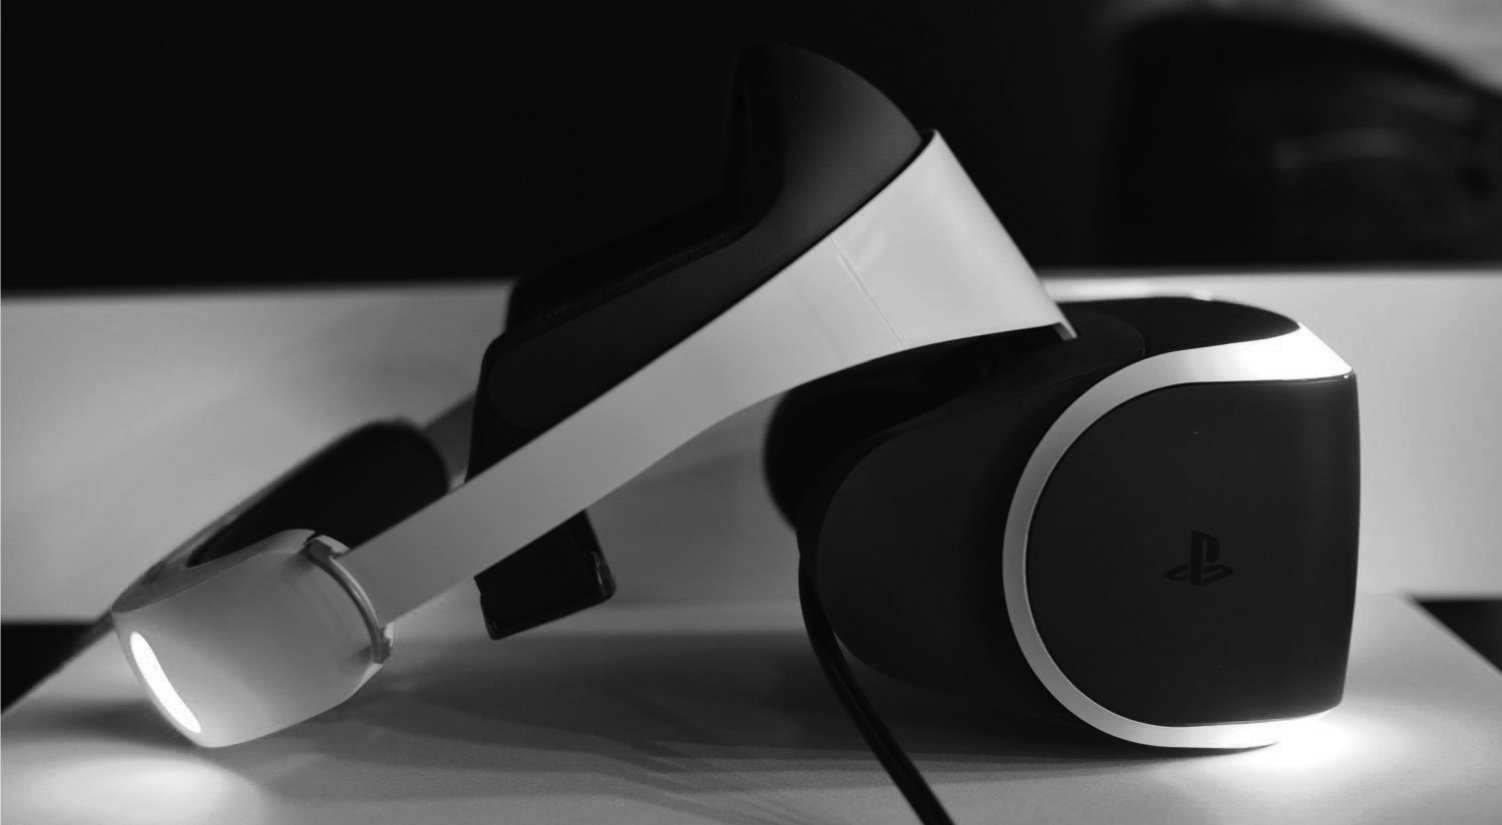
\includegraphics[scale=.5]{img_morpheus}
  %\end{picture}
  \caption{Sony Morpheus prototype seen at the 2015 Games Developer Conference.}
  \label{figure:f_sony_m}
\end{figure}
%Figure~\ref{figure:f_dk1}

Since the release of the DK2, Oculus VR has released a mobile version of their HMD which runs via Android smart phone integration (Samsung Gear VR). In addition, Oculus VR has publicly stated that no further development kits will be released, and instead their next major HMD release will be a full consumer version. There is no confirmation of a release date as of yet.

\subsection{Sony Morpheus}

\begin{figure}
  \centering
  %\begin{picture}
  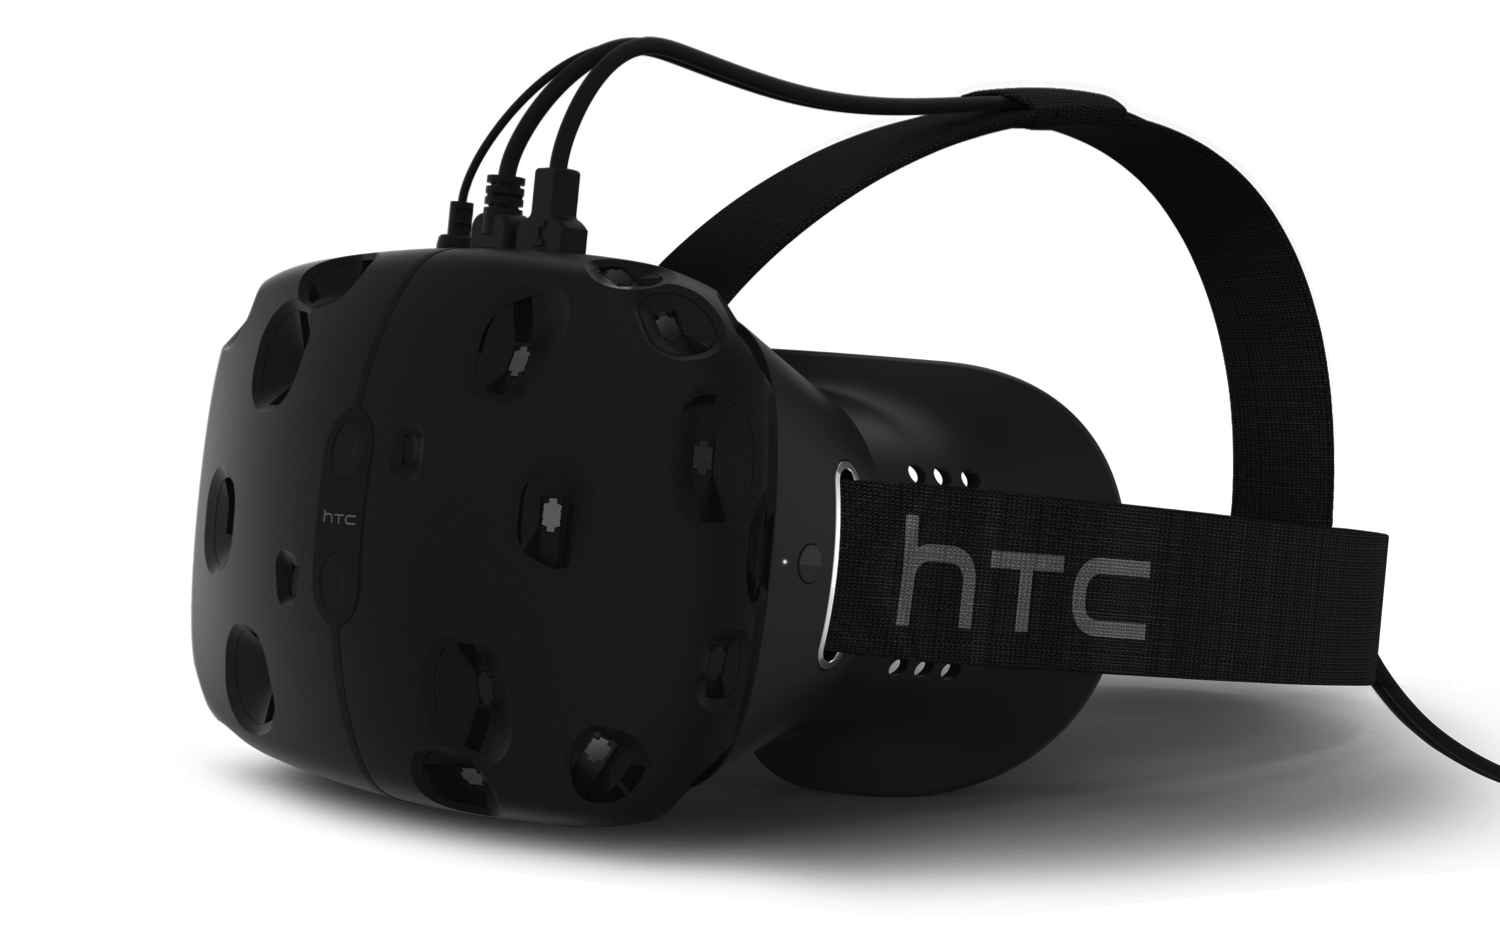
\includegraphics[scale=.5]{img_vive}
  %\end{picture}
  \caption{HTC Vive prototype seen at the 2015 Games Developer Conference.}
  \label{figure:f_vive}
\end{figure}

Oculus VR was of course the first company to truly revolutionize VR tech in today's age, but that is not to say that they are without competitors. Rather, a handful of companies have begun to enter the VR development space and are placing claims on their own HMD technology. One of these companies is the Japanese tech giant Sony, and they have a codenamed HMD known as Project Morpheus in the works. As of the time of writing not much is known about Project Morpheus other than it is an HMD similar to the Oculus Rift that will be fully integrated into PlayStation gaming systems. The HMD is in a prototype stage, however, Sony has been showing the HMD, seen in Figure~\ref{figure:f_sony_m}, at numerous gaming conventions with promises of a consumer release in the first half of 2016.

As far as the actual technical details are concerned, as of writing the latest known specifications for Project Morpheus are quite impressive. For starters, rather than an LCD screen, Sony has decided to use an OLED screen much like the Oculus Rift does. Unlike the Oculus Rift, the frame rate is a massive 120 frames per second, which could help reduce the risk of nausea associated with immersive VR. As well, the total resolution of Project Morpheus is 1920x1080, or 960x1080 per eye, along with a field of view of 100 degrees \cite{kelion_sonys_2015}. 

\subsection{HTC Vive}
\label{sec:valvevr}

Along with Sony, two other companies are making waves in the VR HMD space. These companies are the cell phone hardware manufacturer HTC, and the gaming power house Valve. Even fewer details are available for their prototype HMD as of writing, however, it has been shown recently at gaming conventions, and a potential consumer release could come as early as holiday 2015. The resolution on the HTC Valve HMD, named the HTC Vive, is slightly better than Project Morpheus at 1080x1200 per eye. However, the refresh rate on the HMD is said to be 90 frames per second, significantly lower than Project Morpheus. Yet, the HTC Vive differentiates itself from the competition by relying on two in room base stations which will allow the HTC Vive to track movement within a 15 feet by 15 feet space \cite{kelion_htc_2015}. Figure~\ref{figure:f_vive} demonstrates the futuristic look of the HTC Vive, as it features numerous visible IR sensors across the face plate which differentiates itself from the similarly designed DK2.